\section{\openFortyTwo と\closeFortyTwo のネットワークの比較}
\label{sec:network_comparison}

まず、$\Delta \lambda_{\rm{AB}}$が大きいペアと小さいペアを調べるために、$\Delta \lambda_{\rm{AB}}$ の $\mu \pm 3 \sigma$ よりも小さい、または、大きいペアを抽出した。
図\ref{fig:network_groups_tc_Delta}にドメイン間の$\Delta \lambda_{\rm{AB}}$に着目した図を示す。
また、図\ref{fig:network_groups_tc_Delta_focus_inside}にドメイン内の$\Delta \lambda_{\rm{AB}}$に着目した図を示す。

\begin{figure}
  \centering
  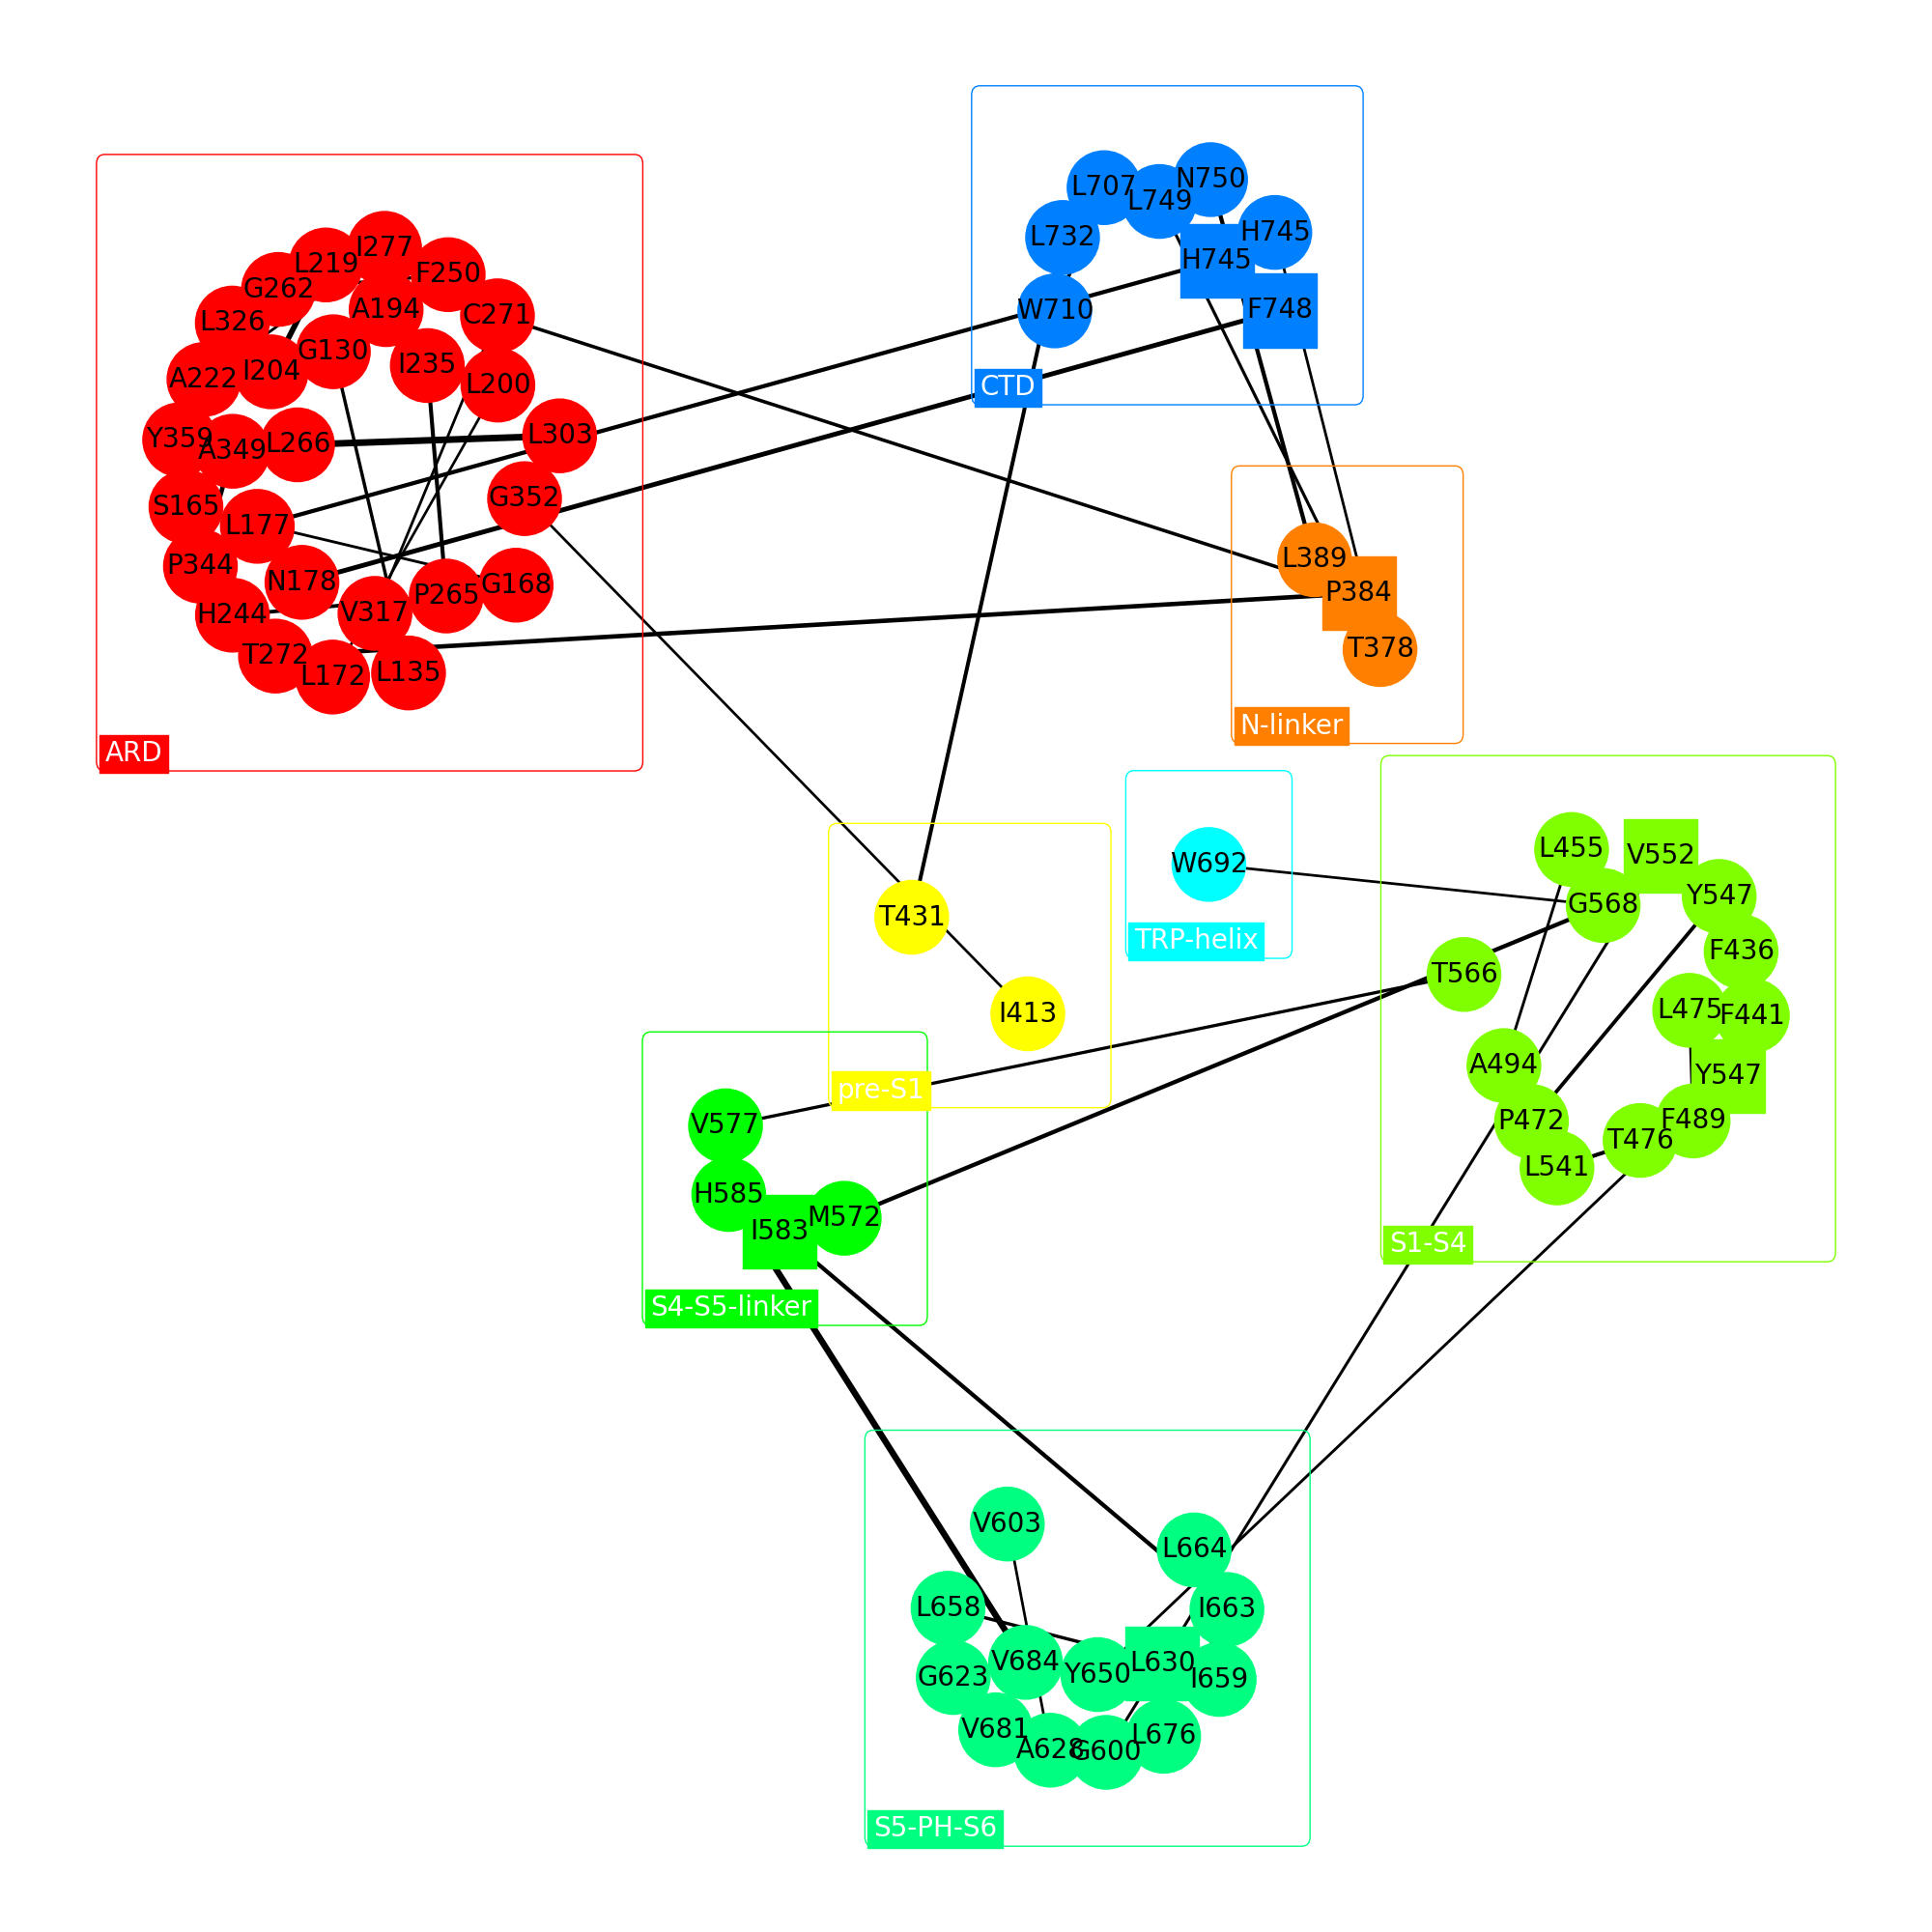
\includegraphics[width=\textwidth]{network_groups_tc_Delta.png}
  \caption{\openFortyTwo と\closeFortyTwo の $\Delta \lambda_{\rm{AB}}$をネットワーク表示した。
            四角形は主鎖Bの残基。ドメインごとに色を分け、N末端側から順にARD、N-linker、pre-S1、S1-S4、S4-S5-linker、S5-PH-S6、TRP-helix、CTDと分けた。
            \autocite{pumroy_structural_2020}}
  \label{fig:network_groups_tc_Delta}
\end{figure}

まず、図\ref{fig:network_groups_tc_Delta}から、
ドメインをさらにグループ化した二つのセグメント、ARD、N-linker、pre-S1、CTDとS1-S4、S4-S5-linker、S5-PH-S6、TRP-helixに分割されていることがわかる。
この分割は、膜より内側部分(ARD、N-linker、pre-S1、CTD)と膜に埋まった部分(S1-S4、S4-S5-linker、S5-PH-S6、TRP-helix)との分割に等しい。
先行研究において、膜より内側の部分におけるARDドメインが熱やリガンドを感受してチャネル開閉を制御する一つの機構であることが示されている\autocite{phelps_differential_2010,phelps_insights_2007,shi_crystal_2013}
にも関わらず、熱流ネットワークにおいて大きな差がみられないことは、興味深い結果である。
おそらくこれらの膜より内側に存在するドメインは、熱を使った仕組みではなく立体配位の変化や膜環境の変化によって情報伝達していると考えられる。
% TRP-helixが立体構造ではPre-S1と近接しているにも関わらず、$\Delta \lambda_{\rm{AB}}$で表したネットワークに表示されないことがわかる。

\begin{figure}
  \centering
  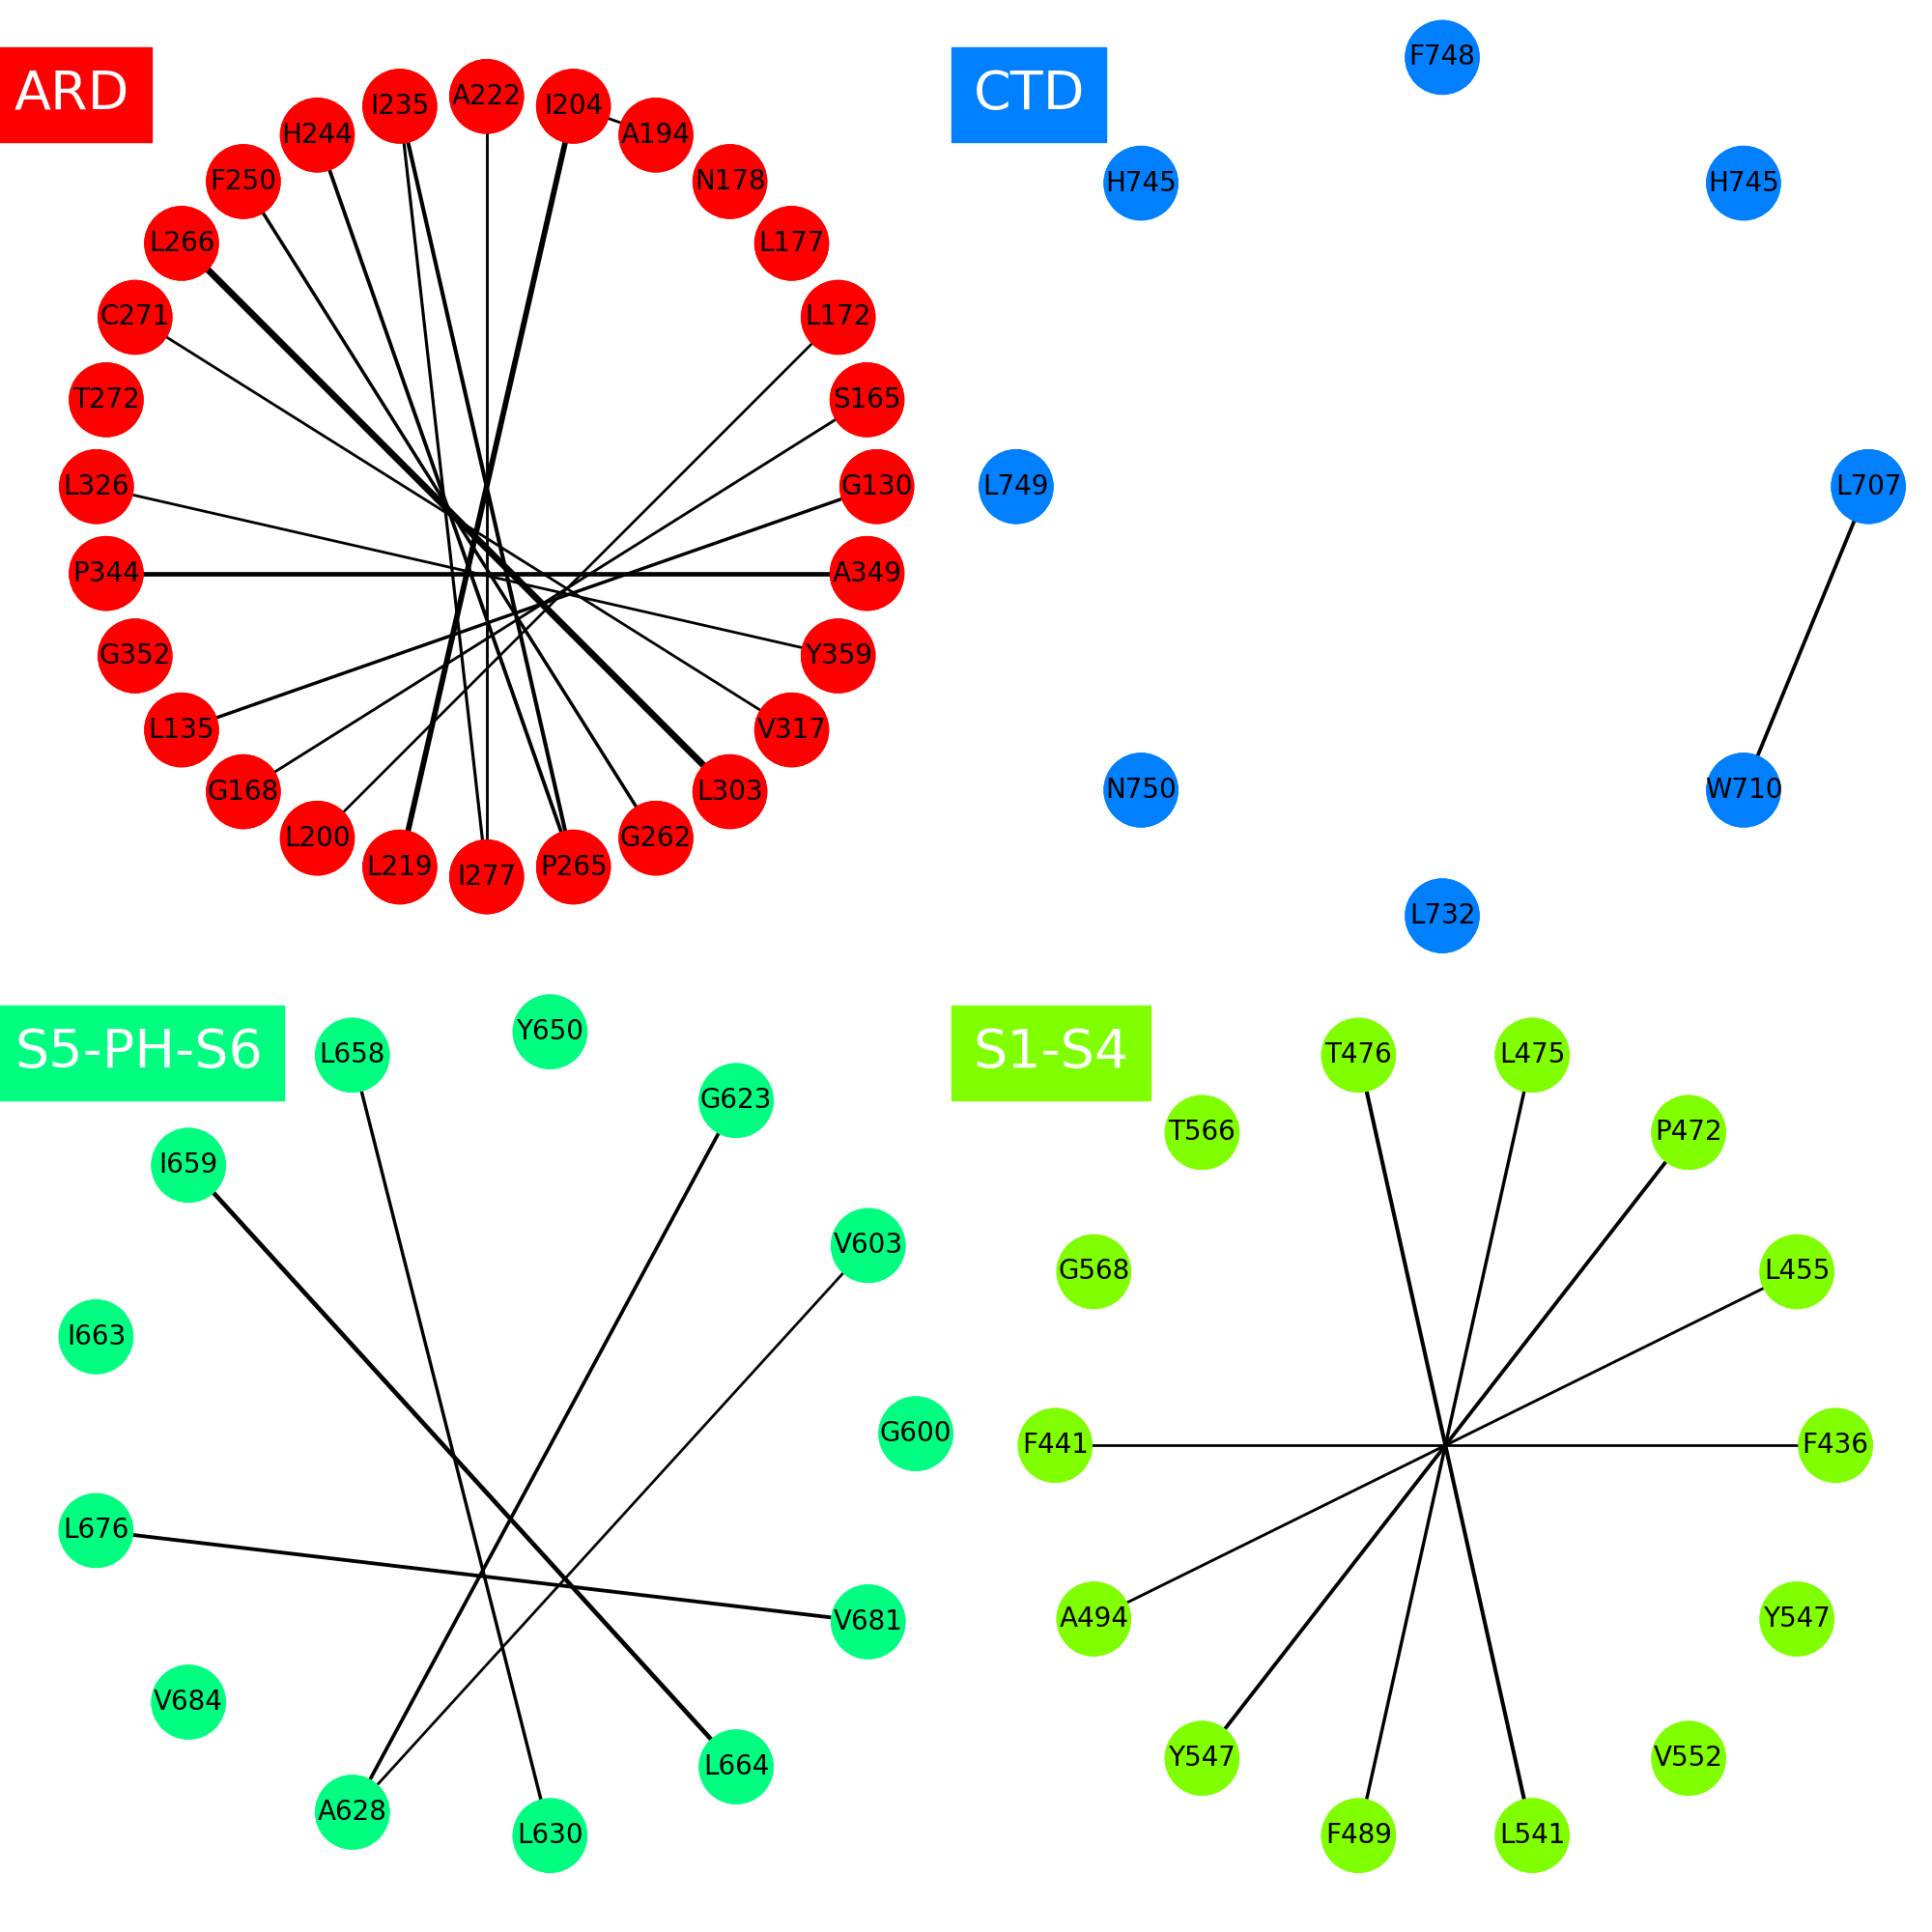
\includegraphics[width=\textwidth]{network_groups_tc_Delta_focus_inside.png}
  \caption{$\Delta \lambda_{\rm{AB}}$が大きいペアのうち、ドメイン内のネットワーク}
  \label{fig:network_groups_tc_Delta_focus_inside}
\end{figure}

\section{機能的に重要な残基}

事前に調査対象としていた機能的に重要と思われる残基について調べた。
\ref{sec:network_comparison}と同様に、$\Delta \lambda_{\rm{AB}}$ の $\mu \pm 3 \sigma$ よりも小さい、または、大きいペアに
表\ref{tab:important_residues}で列挙した残基が含まれているか調べた。
その結果、(G352, I413)間でのみ$\Delta \lambda_{\rm{AB}}$が極端に小さくなる($\Delta \lambda_{\rm{G352},\rm{I413}} < \mu - 3\sigma$)ことがわかった。
I413を変異は刺激が繰り返されることに応じてチャネルの活性が変わるという、TRPV3特有の性質